% LLM-YARA — Rule Rejection Reason Breakdown
% Compile: pdflatex rejection_reasons.tex
\documentclass[border=5pt]{standalone}
\usepackage{tikz}
\usepackage{pgfplots}
\pgfplotsset{compat=1.18}

% ── Colour palette ──────────────────────────────────────────────────
\definecolor{accgreen}{HTML}{16A34A}
\definecolor{accgreenfill}{HTML}{BBF7D0}
\definecolor{warnamber}{HTML}{D97706}
\definecolor{warnamberfill}{HTML}{FDE68A}
\definecolor{errred}{HTML}{DC2626}
\definecolor{errredfill}{HTML}{FECACA}
\definecolor{txtgray}{HTML}{374151}
\definecolor{bggray}{HTML}{F9FAFB}

\begin{document}
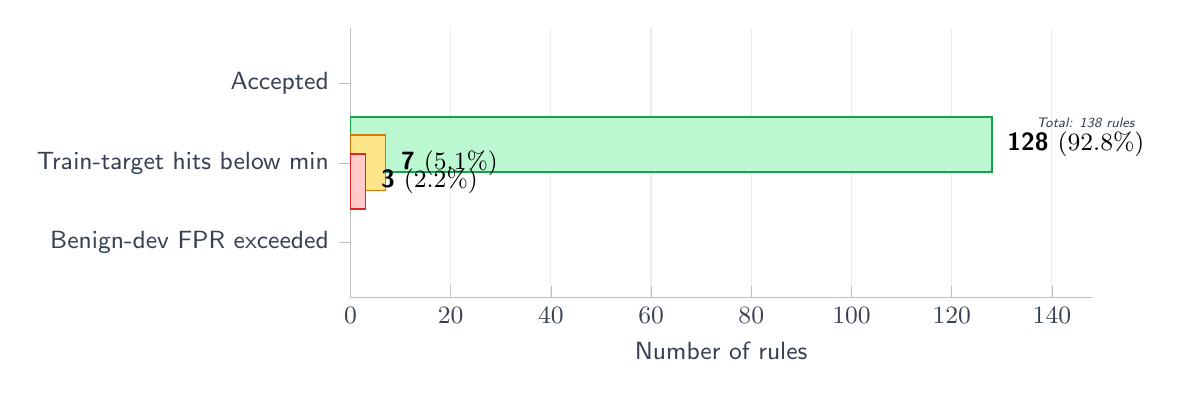
\begin{tikzpicture}
\begin{axis}[
    xbar,
    width=11cm,
    height=5cm,
    bar width=0.7cm,
    xmin=0, xmax=148,
    ytick={1, 2, 3},
    yticklabels={
        {Benign-dev FPR exceeded},
        {Train-target hits below min},
        {Accepted}},
    y tick label style={font=\sffamily\small, text=txtgray, anchor=east},
    x tick label style={font=\sffamily\small, text=txtgray},
    xtick={0, 20, 40, 60, 80, 100, 120, 140},
    xlabel={Number of rules},
    xlabel style={font=\sffamily\small, text=txtgray},
    xmajorgrids=true,
    grid style={gray!15, thin},
    axis line style={gray!50},
    tick style={gray!50},
    axis x line*=bottom,
    axis y line*=left,
    enlarge y limits=0.35,
    clip=false,
    nodes near coords,
    nodes near coords align={horizontal},
    every node near coord/.append style={
        font=\sffamily\small\bfseries,
        anchor=west,
        xshift=2pt,
    },
    point meta=explicit symbolic,
]

% ── Accepted bar ────────────────────────────────────────────────────
\addplot[
    fill=accgreenfill, draw=accgreen, line width=0.6pt,
] coordinates {
    (128, 3) [{128 \textnormal{(92.8\%)}}]
};

% ── Train-target hits below min ─────────────────────────────────────
\addplot[
    fill=warnamberfill, draw=warnamber, line width=0.6pt,
] coordinates {
    (7, 2) [{7 \textnormal{(5.1\%)}}]
};

% ── Benign-dev FPR exceeded ─────────────────────────────────────────
\addplot[
    fill=errredfill, draw=errred, line width=0.6pt,
] coordinates {
    (3, 1) [{3 \textnormal{(2.2\%)}}]
};

% ── Total annotation ────────────────────────────────────────────────
\node[font=\sffamily\tiny, text=txtgray, anchor=west]
    at (axis cs:135, 3) [yshift=-14pt] {\textit{Total: 138 rules}};

\end{axis}
\end{tikzpicture}
\end{document}
